% Style.
\documentclass[letterpaper,portuguese,12pt,pdftex]{exam}

\usepackage{setspace}
\usepackage{lineno}
\usepackage[left=2.5cm,top=3cm,right=2.5cm]{geometry}

% Portuguese.
\usepackage[brazil]{babel}
\usepackage[T1]{fontenc}
\usepackage[utf8x]{inputenc}
\usepackage{textcomp}

% Font.
\usepackage{lmodern}

% Figures.
\usepackage{epsf,epsfig}

% Bibtex and extras.
\usepackage{natbib}
\usepackage{url}
\usepackage[bookmarks=false,colorlinks=true,urlcolor={green},linkcolor={green},pdfstartview={XYZ null null 1.22}]{hyperref}

% Math.
\usepackage{amssymb,amsmath}
\usepackage{mathtools}
\everymath{\displaystyle}

% Exam.
\addpoints
\printanswers
% \noprintanswers
\usepackage{color}
\definecolor{SolutionColor}{rgb}{0.8,0.9,1}
\shadedsolutions
\renewcommand{\solutiontitle}{\noindent\textbf{Solução:}\par\noindent}
\pagestyle{headandfoot}
\footer{}{Página \thepage\ de \numpages}{}
\boxedpoints
\pointsinrightmargin
\pointpoints{ponto}{pontos}
\hqword{Questão}
\hpword{Pontos}
\hsword{Nota}
% \qformat{\textbf{Question\thequestion}\quad(\thepoints)\hfill}

% User commands.
\newcommand{\pd}[2]{\frac{\partial #1}{\partial #2}}

% PDF metadata.
\pdfinfo{% hyperref overrides this
  /Title    (Lista 05 -- Oceanografia Física Descritiva)
  /Author   (Filipe Fernandes)
  /Creator  (Filipe Fernandes)
  /Producer (Filipe Fernandes)
  /Subject  (Lista)
  /Keywords (Lista, oceanografia)
}

% Front page.
\title{Lista 05 -- Oceanografia Física Descritiva}
\author{Prof. Filipe Fernandes}
\date{23-Sep-2013}

\begin{document}
\maketitle
\doublespacing

\begin{minipage}{.8\textwidth}
Essa lista incluí \numquestions\ questões. O número total de pontos é \numpoints.
\end{minipage}
\vspace{0.5cm}

% 25
\begin{questions}

\question
Imagine que duas massas d'água com $\theta$=2 \textcelsius, S=35.04 g/kg e
$\theta$=8.5\textcelsius, S=36.00 g/kg se misturam em proporções
aproximadamente iguais.

\begin{figure}[ht]
  \centering
%   \includegraphics[scale=0.7]{./figures/diagrama_TS.pdf}
  \includegraphics[scale=0.7]{./solution/Diagrama-TS.pdf}
  \label{fig:TS}
  \caption{Diagrama TS}
\end{figure}

\begin{parts}

  \part[1]
  \label{qt:denso}
  Plote no diagrama TS fornecido (\ref{fig:TS}) as duas massas d'água originais
  e a formada pela mistura.  O que é particularmente interessante dessa mistura?

\begin{solution}
      $\theta$=5.25, S = 35.52 g/kg
  \end{solution}

  \begin{solution}
    Essa massa d'água é mais densa que as duas que a formaram.  Mostrando a não
    linearidade da equação de estado.
  \end{solution}

  \part[1]
  Usando a forma para a equação de estado:

  \begin{equation}
    \rho = \rho_o - \underbrace{\alpha(T - T_o)}_{a} +
           \underbrace{\beta(S-S_o)}_b + \underbrace{\kappa p}_c
    \label{eq:linear}
  \end{equation}

  Explique os termos $a$, $b$ e $c$.  As linhas de densidade da figura
  \ref{fig:TS} foram desenhadas usando a equação acima?  É possível estudarmos o
  efeito observado na sua reposta do item \ref{qt:denso} com essa equação?
  (Explique a sua resposta.)

  \begin{solution}
  $a$: Expansão térmica.

  $b$: Contração Salina.

  $c$: Compressão bárica.
  \end{solution}

  \begin{solution}
  Não para ambos.  As linhas foram desenhadas utilizando a forma não linear da equação
  do estado.
  \end{solution}
\end{parts}

\question
 Usando a equação \ref{eq:linear} fornecida no exercício anterior corte o termo
 referente a pressão e faça a derivada parcial com relação à salinidade e a
 derivada parcial com relação à temperatura:
 \begin{parts}
  \part[1]
  $\pd{\rho}{S} = $

  \vspace{0.5cm}

  $\pd{\rho}{T} = $

  \begin{solution}
  $\pd{\rho}{S} \equiv \beta \delta S$

  $\pd{\rho}{T} \equiv -\alpha \delta T$
  \end{solution}

  \part[1]
  Usando $\alpha = 0.15$ kg m$^{-3} \text{\textcelsius}^{-1}$ e
  $\beta = 0.78$ kg m$^{-3}$ (g/kg)$^{-1}$

  Calcule qual a variação de salinidade necessária para aumentar a densidade em
  1 kg m$^{-3}$ a temperatura constante.  E qual a variação de temperatura
  necessária para o mesmo aumento de 1 kg m$^{-3}$ a salinidade constante?  (Comente a sua resposta.)

  \begin{solution}
  $\delta \rho \approx \beta \delta S = 1/0.78 = 1.28$ g/kg

  $\delta \rho \approx -\alpha \delta T = 1/-0.15 = -6.66$\textcelsius
  \end{solution}

  \part[1]
  Esquematize um perfil oceânico de temperatura, salinidade e densidade típico
  para regiões sub-tropicais e nomeie as 3 camadas de estratificação que
  conhecemos.  Com base na sua resposta acima explique a variação de densidade
  em  função da temperatura e da salinidade.

  \begin{solution}
  O perfil de densidade é quase um espelho da temperatura porque, apesar da
  densidade variar mais com a salinidade, a variação da temperatura é muito
  maior.
  \end{solution}

  \part[1]
  Comente a sua resposta acima caso os perfis fossem em regiões polares.  Fale
  sobre as semelhanças e diferenças.

  \begin{solution}
  Em regiões polares a temperatura varia muito pouco, sendo a coluna d'água
  estratificada pela salinidade.
  \end{solution}

 \end{parts}

\question
Propriedades conservativas.

 \begin{parts}
  \part[1]
  Explique os termos da equação:
  $$\underbrace{\pd{S}{t}}_a = \underbrace{\vec{u}\nabla S}_b + \underbrace{\phi}_c$$

  \begin{solution}
  $a$: Variação local de salinidade.

  $b$: Salinidade transportada para o sistema.

  $c$: Fonte ou sorvedouro de salinidade.
  \end{solution}

  \part[1]
  Cite duas condições por trás da análise de massas d'água.
  \begin{solution}
  1) T e S tem que ser conservativos, longe da superfície.

  2) A mistura das massas d'água se da  na mesma proporção.
  \end{solution}

 \end{parts}

\question[2]
Usando a figura (\ref{fig:termo}), que mostra a variação de temperatura em
uma região temperada do hemisfério Sul, responda.

\begin{figure}[ht]
  \centering
  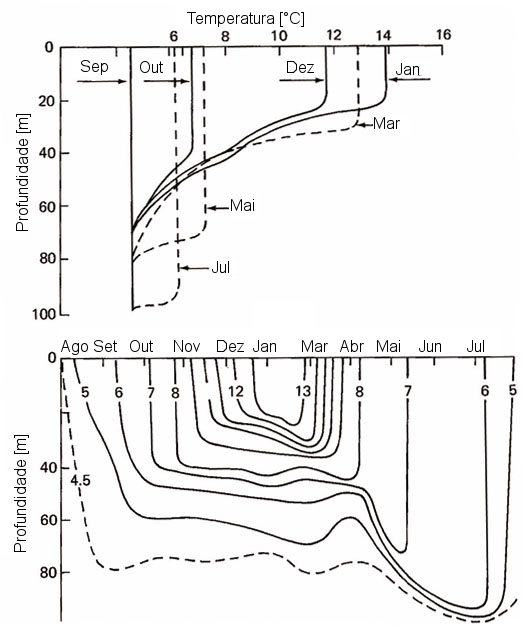
\includegraphics{./figures/termoclina_sazonal.png}
  \caption{Painel superior: Diversos perfis de temperatura ao longo de um ano.
           Painel inferior: Seção vertical de temperatura ao longo do ano.}
  \label{fig:termo}
\end{figure}

  Observe o painel superior da figura e explique a formação e erosão da
  termoclina sazonal.

  \begin{solution}
  {\bf Primavera (Setembro, Outubro, Novembro):}

  Com a chegada da primavera o perfil pouco estratificado se torna aos poucos
  mais estratificado com o aquecimento da superfície começando a formação de uma
  termoclina sazonal sobre a termoclina permanente.

  {\bf Verão (Dezembro, Janeiro, Fevereiro):}

  No verão a superfície do oceano se encontra estabilizada e o perfil apresenta
  uma redução da camada de mistura em função do aquecimento.

  {\bf Outono (Março, Abril, Maio):}

  Com o resfriamento das camadas de superfície a camada superior fica instável
  e a camada de mistura aumenta avançando sobre a termoclina sazonal.

  {\bf Inverno (Junho, Julho, Agosto):}

  A termoclina sazonal é quase completamente erodida e a camada de mistura
  se encontra com a termoclina permanente.
  \end{solution}

\end{questions}

\end{document}
